% Emotion Intensity
\begin{table}[t]
\centering
\small
\resizebox{\linewidth}{!}{
\setlength{\tabcolsep}{3pt}
\begin{tabular}{l|ccccc}
\toprule
Methods & PSNR$\uparrow$ & LMD$\downarrow$ & \multicolumn{2}{c}{AUE-(L/U)$\downarrow$} & Sync-C$\uparrow$ \\
\midrule
\multicolumn{6}{c}{\textbf{Level-1 (Weaker Intensity)}} \\
\midrule
Real3DPortrait~\cite{ye2024real3d} & 25.27 & 3.581 & 1.148 & 1.094 & \textbf{6.593} \\
MimicTalk~\cite{ye2024mimictalk}     & 25.18 & 3.504 & \underline{0.946} & 0.895 & 6.129 \\
InsTaG~\cite{li2025instag}              & \underline{28.03} &\underline{3.352} & 0.968 & \underline{0.613} & 5.014 \\
\rowcolor{gray!20} \textbf{EmoTaG (Ours)}                  & \textbf{30.01} & \textbf{2.367} & \textbf{0.697} & \textbf{0.221} & \underline{6.154} \\
\midrule
\multicolumn{6}{c}{\textbf{Level-3 (Stronger Intensity)}} \\
\midrule
Real3DPortrait~\cite{ye2024real3d} & 25.11 & 3.742 & 1.215 & 1.238 & \textbf{6.585} \\
MimicTalk~\cite{ye2024mimictalk}      & 25.05 & 3.637 & \underline{0.981} & 0.933 & 6.118 \\
InsTaG~\cite{li2025instag}              & \underline{27.56} & \underline{3.559} & 1.144 & \underline{0.704} & 4.637 \\
\rowcolor{gray!20} \textbf{EmoTaG (Ours)}                  & \textbf{29.92} & \textbf{2.522} & \textbf{0.721} & \textbf{0.244} & \underline{6.126} \\
\bottomrule
\end{tabular}
}
\vspace{-5pt}
\caption{
\textbf{Quantitative comparison on \textit{emotion-intensity}.} We adapt models on Level-2 (medium) and test on Level-1 (weaker) and Level-3 (stronger) separately.
[Key: \textbf{Best}, \underline{Second Best}]}
\vspace{-10pt}
\label{tab:emotion_intensity}
\end{table}


\section{Experiment}

\textbf{Datasets.}
We train EmoTaG on the HDTF dataset~\cite{zhang2021flow}, using 70 videos (90-240 seconds each) from 70 identities to learn identity-agnostic audio-motion priors. For evaluation, we construct two test sets: a neutral set comprising 10 public videos of 10 identities from~\cite{li2023efficient, ye2023geneface}, and an emotional set derived from MEAD~\cite{wang2020mead}, covering 5 emotion categories-\textit{happy}, \textit{sad}, \textit{surprised}, \textit{angry}, and \textit{fear}-with 3 intensity levels and 2 identities per emotion. All videos are face-centered cropped and resized to $512{\times}512$ at 25 FPS.


\noindent \textbf{Baselines.}
We compare EmoTaG with representative 3D talking-head baselines across different training settings.
Train-from-scratch methods include ER-NeRF~\cite{li2023efficient} and TalkingGaussian~\cite{li2024talkinggaussian}, which require full retraining per identity.
In the one-shot setting, we evaluate Real3DPortrait~\cite{ye2024real3d}, which enables rapid identity initialization from a single reference image.
For few-shot adaptation, we compare against GeneFace++~\cite{ye2023geneface++}, MimicTalk~\cite{ye2024mimictalk}, and InsTaG~\cite{li2025instag}.
All baselines are reproduced using their official implementations, with Wav2Vec~2.0~\cite{baevski2020wav2vec} as the unified audio feature extractor for fair comparison.

\noindent \textbf{Metrics.}
We evaluate EmoTaG in terms of rendering fidelity, motion accuracy, lip synchronization, and efficiency.
Image quality is assessed using PSNR, SSIM~\cite{wang2004image}, and LPIPS~\cite{zhang2018unreasonable} between rendered and ground-truth frames.
Facial-motion accuracy is measured by Landmark Distance (LMD) and Action Unit Error for the lower face and upper face (AUE-L/U)~\cite{ekman1978facial, li2024talkinggaussian}.
Audio-visual synchronization is quantified with SyncNet-based Confidence (Sync-C) and Error (Sync-E)~\cite{chung2016lip, chung2016out}.
Efficiency is reported in terms of training time and inference FPS.

\noindent \textbf{Implementation Details.}
We employ VHAP~\cite{qian2024vhap} as our FLAME tracker to obtain the FLAME shape parameters, non-jaw head pose, and camera parameters. The 3D Gaussian field is initialized with 60K Gaussians uniformly sampled from the FLAME mesh. Training follows a two-stage curriculum. For each identity, the first 1,000 iterations optimize static appearance only, after which Gaussian parameters and the Gated Residual Motion Network are jointly optimized. Pretraining and adaptation are performed for $250$K and $20$K iterations, respectively, using AdamW~\cite{loshchilov2017decoupled} with learning rates of $5{\times}10^{-3}$ and $5{\times}10^{-4}$, correspondingly. Loss weights are set to $\lambda_{\text{D-SSIM}}{=}2{\times}10^{-1}$, $\lambda_{D}{=}1{\times}10^{-2}$, and $\lambda_{N}{=}1{\times}10^{-3}$. All experiments are conducted on a single NVIDIA RTX~A6000 GPU. In our method, audio encoding is performed once per sequence ($\sim$25 ms), and each frame requires $\sim$6 ms for GRMN inference and $\sim$7 ms for 3DGS rendering. Additional implementation details are provided in the supplementary material.

%-------------------------------------------------------------------------
\subsection{Evaluation}
\textbf{Comparison Settings.} 
We evaluate EmoTaG under three settings: (1) \textit{Self-reconstruction}, where each model is adapted on a 5-second video and evaluated on another clip (3-10 seconds) of the same emotion and identity, measuring few-shot rendering quality, motion accuracy, and lip synchronization.
(2) \textit{Emotion-intensity}, where models adapted on Level-2 are tested on Level-1 and Level-3 audio of the same emotion and identity to assess sensitivity to intensity variation.
(3) \textit{Out-of-distribution (OOD) audio-driven}, which evaluates generalization to unseen audio while keeping the adapted identity fixed. We consider (a) cross-identity—speech from a different speaker in the same language, and (b) cross-language—speech in a different language from the adaptation clip. For each case, we sample three audio clips from public videos.
Following the prior work~\cite{li2025instag}, we use pose \& expression cues from the test clip for \textit{self-reconstruction} and \textit{emotion-intensity} settings, and from the adaptation clip for \textit{OOD audio-driven}.


% Cross domain
\begin{table}[t]
\centering
\small
\resizebox{\linewidth}{!}{
\setlength{\tabcolsep}{3pt}
\begin{tabular}{l|cc|cc}
\toprule
\multirow{2}{*}{Methods} &
\multicolumn{2}{c|}{\textit{Cross Identity}} &
\multicolumn{2}{c}{\textit{Cross Language}} \\
& \makecell{Sync-E $\downarrow$} 
& \makecell{Sync-C $\uparrow$} 
& \makecell{Sync-E $\downarrow$} 
& \makecell{Sync-C $\uparrow$} \\
\midrule
ER-NeRF~\cite{li2023efficient}          & 11.732 & 2.833 & 11.931 & 2.542 \\
GeneFace++~\cite{ye2023geneface++}      & 10.515 & 3.497 &  11.052  & 3.107 \\
TalkingGaussian~\cite{li2024talkinggaussian} & 10.407 & 3.207 & 10.938 & 2.941 \\
InsTaG~\cite{li2025instag}        & \underline{9.921} & \underline{4.722} & \underline{10.033} & \underline{4.391} \\
\midrule
\textbf{EmoTaG (Ours)}         & \textbf{9.133} & \textbf{5.814} & \textbf{9.662} & \textbf{5.432} \\
\bottomrule
\end{tabular}
}
\vspace{-5pt}
\caption{
\textbf{Quantitative results of lip synchronization on \textit{OOD audio-driven}.} 
We evaluate two challenging scenarios: \textit{cross-identity} and \textit{cross-language}. 
[Key: \textbf{Best}, \underline{Second Best}]}
\vspace{-10pt}
\label{tab:cross_domain}
\end{table}

\noindent \textbf{Quantitative Results.}
Tab.~\ref{tab:main} reports the \textit{self-reconstruction} results.
Across both neutral and emotional test sets, EmoTaG achieves the best overall performance, with the highest PSNR/SSIM and lowest LPIPS, indicating superior appearance fidelity and geometric stability. Its lowest LMD and AUE-(L/U) further reflect accurate lip articulation and natural upper-face motion. Although EmoTaG is not the best on Sync-C, it remains close to the two large-scale pretrained models~\cite{ye2024real3d, ye2024mimictalk} and substantially outperforms them on the remaining metrics. EmoTaG adapts in 11 minutes and runs in real time at 76.4~FPS.
Tab.~\ref{tab:emotion_intensity} evaluates \textit{emotion-intensity} sensitivity.
When adapted on Level-2 and tested on Level-1/Level-3, EmoTaG obtains the lowest LMD and AUE-(L/U), demonstrating precise modulation across intensity levels while maintaining competitive Sync-C and the highest visual quality. Notably, its performance gains over InsTaG are larger at higher intensity, highlighting greater robustness to intense emotions.
In the \textit{out-of-distribution} evaluation (Tab.~\ref{tab:cross_domain}), EmoTaG achieves the lowest Sync-E and highest Sync-C in both \textit{cross-identity} and \textit{cross-language} settings, confirming better audio-motion generalization and lip synchronization under unseen speakers and languages.

\noindent \textbf{Qualitative Comparison.}
Fig.~\ref{fig:Qual_Results} presents qualitative comparisons under the \textit{self-reconstruction} setting. 
Compared with existing approaches, EmoTaG produces more expressive results with stable identity preservation. 
TalkingGaussian~\cite{li2024talkinggaussian} exhibits visible artifacts and mouth-audio misalignment, while InsTaG~\cite{li2025instag} improves lip synchronization but lacks natural emotional variation. 
MimicTalk~\cite{ye2024mimictalk} and Real3DPortrait~\cite{ye2024real3d} achieve better alignment due to large-scale pretraining yet still generate rigid and over-smoothed expressions. 
Using strong structural priors and emotion-aware motion learning, EmoTaG reconstructs photorealistic details and consistent facial dynamics in both neutral and emotional tests. 
We strongly recommend viewing the supplementary video for dynamic comparison.

% User Study
\begin{table}[t]
\centering
\small
\resizebox{\linewidth}{!}{
\setlength{\tabcolsep}{3pt}
\begin{tabular}{l|ccc}
\toprule
Method & Emo Expr & Lip Sync & Visual Realism \\
\midrule
Real3DPortrait~\cite{ye2024real3d} & 2.20 & 3.50 & 3.20 \\
TalkingGaussian~\cite{li2024talkinggaussian}             & 3.30 & 2.40 & 3.00 \\
MimicTalk~\cite{ye2024mimictalk}             & 3.50 & \underline{4.10} & 3.70 \\
InsTaG~\cite{li2025instag}     & \underline{3.80} & 3.90 & \underline{4.20} \\
\midrule
\textbf{EmoTaG (Ours)}                & \textbf{4.50} & \textbf{4.70} & \textbf{4.60} \\
\bottomrule
\end{tabular}
}
\vspace{-5pt}
\caption{
\textbf{User study on emotional expressiveness, lip synchronization, and visual realism.} 
Ratings range from 1 to 5, where higher indicates better performance. 
[Key: \textbf{Best}, \underline{Second Best}]}
\vspace{-10pt}
\label{tab:user-study}
\end{table}

\noindent \textbf{User Study.}
To assess perceptual quality, we conduct a user study comparing EmoTaG against representative baselines.
Twenty participants rate anonymized results from the \textit{self-reconstruction} setting on emotional expressiveness, lip synchronization, and visual realism (1-5 Likert, higher is better).
As shown in Tab.~\ref{tab:user-study}, EmoTaG achieves the best overall scores, notably on emotional expressiveness, demonstrating stronger emotion-aware and coherent facial motion.


%-------------------------------------------------------------------------
\subsection{Ablation Study}
To evaluate the contribution of each component, we ablate by removing key modules of EmoTaG. Quantitative results are listed in Tab.~\ref{tab:ablation}, and qualitative examples are in Fig.~\ref{fig:ablation}.  

\noindent \textbf{Semantic Emotion Guidance (SEG).}  
Removing SEG leads to a consistent degradation across all evaluation metrics, underscoring its crucial role in enabling emotion-aware audio-motion mapping.
A deeper look into its components reveals that removing $\mathcal{L}_{\text{Score}}$ primarily harms audio-motion synchronization due to unstable motion representation, whereas removing $\mathcal{L}_{\text{KL}}$ results in more significant decline in both motion accuracy and visual fidelity, since the residual branch loses its semantic guidance for modeling emotion-driven deformation patterns. 

\noindent \textbf{Expert Motion Decoder.}  
Removing the gate branch introduces temporal instability and weakens audio-motion synchronization.
Disabling the residual branch yields oversmoothed and less expressive motion due to the loss of fine-grained emotional variation.
Eliminating AdaIN-based identity modulation causes the largest performance drop, indicating that it is crucial for preserving identity-specific motion and stabilizing pretraining, without which learning becomes substantially more entangled across identities.

% Ablation Study Table
\begin{table}[t]
\centering
\small
\resizebox{\linewidth}{!}{
\setlength{\tabcolsep}{4pt}
\begin{tabular}{l|cccc}
\toprule
\textbf{Variant} & PSNR$\uparrow$ & LPIPS$\downarrow$ & LMD$\downarrow$ & Sync-C$\uparrow$ \\
\midrule
\textbf{EmoTaG (Full Model)}        &  \textbf{29.95} &  \textbf{0.022} &  \textbf{2.456} &  \textbf{6.147} \\
\midrule
\quad w/o Score Distill ($\mathcal{L}_{\text{Score}}$)  & 29.52 & 0.026 & 2.731 & 5.874 \\
\quad w/o KL Distill ($\mathcal{L}_{\text{KL}}$)        & 29.36 & 0.031 & 2.985 & 5.712 \\
\quad w/o SEG                    & 29.01 & 0.034 & 3.067 & 5.541 \\
\midrule
\quad w/o Gate Branch                                    & 28.77 & 0.036 & 3.358 & 5.004 \\
\quad w/o Residual Branch                                & 28.52 & 0.038 & 3.572 & 4.896 \\
\quad w/o Identity Modulation (AdaIN)                   & 28.38 & 0.040 & 4.021 & 4.621 \\
\bottomrule
\end{tabular}
}
\vspace{-5pt}
\caption{
\textbf{Ablation study of EmoTaG.} 
Evaluated under the 5s \textit{self-reconstruction} setting on the emotional test set, showing the effect of each component on quality and synchronization.
}
\vspace{-6pt}
\label{tab:ablation}
\end{table}

% Ablation Study Figure
\begin{figure}[t] 
\centering 
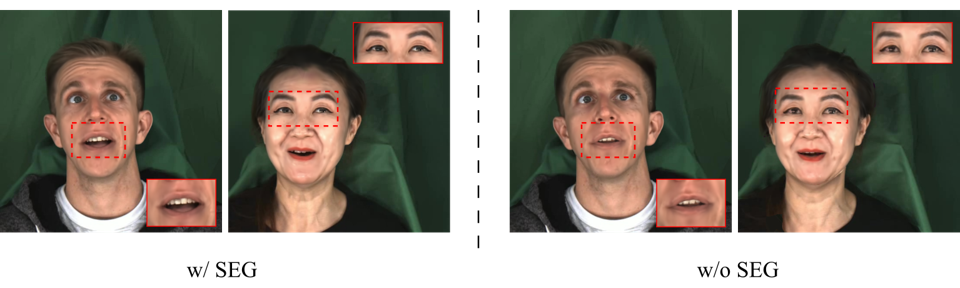
\includegraphics[width=\linewidth]{./Fig/ablation_SEG.png} 
\vspace{-20pt}
\caption{
\textbf{Effect of Semantic Emotion Guidance (SEG).} 
SEG enhances upper-face expressiveness and audio-emotion coherence compared to the model without it.} 
\vspace{-10pt}
\label{fig:ablation} 
\end{figure}